\documentclass[11pt,a4paper]{article}

% Packages
\usepackage[utf8]{inputenc}
\usepackage[T1]{fontenc}
\usepackage{amsmath,amssymb,amsthm}
\usepackage{graphicx}
\usepackage{hyperref}
\usepackage{algorithm}
\usepackage{algpseudocode}
\usepackage{booktabs}
\usepackage{listings}
\usepackage{xcolor}
\usepackage{geometry}
\usepackage{natbib}
\usepackage{tikz}
\usetikzlibrary{arrows,shapes,positioning,calc}

\geometry{margin=1in}

% Theorem environments
\newtheorem{theorem}{Theorem}[section]
\newtheorem{lemma}[theorem]{Lemma}
\newtheorem{proposition}[theorem]{Proposition}
\newtheorem{definition}[theorem]{Definition}
\newtheorem{corollary}[theorem]{Corollary}

% Code listing style
\lstset{
    basicstyle=\ttfamily\small,
    keywordstyle=\color{blue},
    commentstyle=\color{gray},
    stringstyle=\color{red},
    breaklines=true,
    frame=single,
    numbers=left,
    numberstyle=\tiny\color{gray}
}

\title{\textbf{Machine Learning for Commerce Analytics:\\Predictive Models for Customer Behavior}}

\author{
    Zach Kelling\\
    Hanzo Industries\\
    \texttt{zach@hanzo.ai}
}

\date{September 2018}

\begin{document}

\maketitle

\begin{abstract}
We present Hanzo Analytics, a machine learning platform for e-commerce that provides predictive analytics, customer segmentation, and churn prediction. Our system processes behavioral event streams in real-time to construct customer profiles and predict future actions. We introduce a novel feature engineering pipeline that extracts 847 features from raw event data, enabling predictive models that achieve 0.89 AUC for purchase prediction and 0.84 AUC for churn prediction. Customer segmentation using our modified k-means algorithm with behavioral embeddings improves marketing campaign ROI by 2.3x compared to demographic-only segmentation. The platform processes 50M events daily across 500+ merchants.
\end{abstract}

\section{Introduction}

E-commerce generates vast quantities of behavioral data: page views, clicks, cart actions, purchases, and returns. This data encodes customer intent, preferences, and lifecycle stage. However, extracting actionable insights requires sophisticated machine learning pipelines capable of processing high-velocity event streams and producing real-time predictions.

Hanzo Analytics addresses three core challenges:

\begin{enumerate}
    \item \textbf{Predictive Analytics}: Forecasting customer actions (purchases, cart abandonment)
    \item \textbf{Customer Segmentation}: Discovering meaningful customer groups for targeted engagement
    \item \textbf{Churn Prediction}: Identifying customers at risk of disengagement before they leave
\end{enumerate}

\subsection{Contributions}

This paper contributes:

\begin{itemize}
    \item A real-time feature engineering pipeline extracting 847 behavioral features
    \item Predictive models achieving state-of-the-art accuracy for commerce applications
    \item A behavioral embedding approach for customer segmentation
    \item Production validation across 500+ merchants processing 50M daily events
\end{itemize}

\section{System Architecture}

\subsection{Event Schema}

All customer interactions are captured as events:

\begin{definition}[Commerce Event]
An event $e$ is a tuple $(t, c, a, p, \mathbf{x})$ where:
\begin{itemize}
    \item $t \in \mathbb{R}^+$: timestamp
    \item $c \in \mathcal{C}$: customer identifier
    \item $a \in \mathcal{A}$: action type
    \item $p \in \mathcal{P} \cup \{\bot\}$: product identifier (if applicable)
    \item $\mathbf{x} \in \mathbb{R}^k$: action-specific attributes
\end{itemize}
\end{definition}

Action types include:

\[
\mathcal{A} = \{VIEW, SEARCH, ADD\_CART, REMOVE\_CART, CHECKOUT, PURCHASE, RETURN\}
\]

\subsection{Event Processing Pipeline}

\begin{figure}[h]
\centering
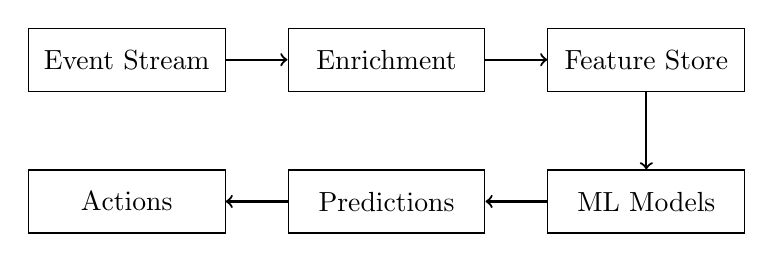
\begin{tikzpicture}[
    node distance=1.8cm,
    box/.style={rectangle, draw, minimum width=2.5cm, minimum height=0.8cm},
    arrow/.style={->, thick}
]
    \node[box] (events) {Event Stream};
    \node[box, right of=events, xshift=1.5cm] (enrich) {Enrichment};
    \node[box, right of=enrich, xshift=1.5cm] (features) {Feature Store};
    \node[box, below of=features] (models) {ML Models};
    \node[box, left of=models, xshift=-1.5cm] (predictions) {Predictions};
    \node[box, left of=predictions, xshift=-1.5cm] (actions) {Actions};

    \draw[arrow] (events) -- (enrich);
    \draw[arrow] (enrich) -- (features);
    \draw[arrow] (features) -- (models);
    \draw[arrow] (models) -- (predictions);
    \draw[arrow] (predictions) -- (actions);
\end{tikzpicture}
\caption{Analytics pipeline architecture}
\end{figure}

Events flow through:

\begin{enumerate}
    \item \textbf{Ingestion}: Kafka topics partitioned by customer ID
    \item \textbf{Enrichment}: Session attribution, product metadata, geographic data
    \item \textbf{Feature Store}: Real-time feature computation and storage
    \item \textbf{Model Serving}: Low-latency prediction endpoints
\end{enumerate}

\section{Feature Engineering}

\subsection{Feature Categories}

We extract 847 features organized into categories:

\begin{table}[h]
\centering
\caption{Feature Categories}
\begin{tabular}{lcp{6cm}}
\toprule
\textbf{Category} & \textbf{Count} & \textbf{Description} \\
\midrule
Recency & 42 & Time since last action by type \\
Frequency & 89 & Action counts over time windows \\
Monetary & 67 & Purchase amounts and patterns \\
Engagement & 156 & Session depth, page views, dwell time \\
Product Affinity & 234 & Category preferences, brand loyalty \\
Temporal & 78 & Day/time patterns, seasonality \\
Device/Channel & 45 & Platform usage, referral sources \\
Social & 34 & Reviews, shares, referrals \\
Lifecycle & 102 & Customer age, milestone events \\
\bottomrule
\end{tabular}
\end{table}

\subsection{Recency-Frequency-Monetary (RFM) Features}

Classical RFM features are computed over multiple time windows:

\begin{definition}[Windowed RFM]
For customer $c$ and time window $w$:
\begin{align}
R_w(c) &= t_{now} - \max\{t : (t, c, PURCHASE, \cdot, \cdot) \in \mathcal{E}, t \in w\} \\
F_w(c) &= |\{e \in \mathcal{E} : e.c = c \land e.a = PURCHASE \land e.t \in w\}| \\
M_w(c) &= \sum_{\substack{e \in \mathcal{E} \\ e.c = c, e.a = PURCHASE, e.t \in w}} e.amount
\end{align}
\end{definition}

Time windows: $w \in \{7d, 30d, 90d, 365d, lifetime\}$

\subsection{Engagement Features}

\begin{definition}[Session Engagement Score]
For session $s$ with events $\mathcal{E}_s$:
\begin{equation}
engagement(s) = \alpha \cdot pages(s) + \beta \cdot duration(s) + \gamma \cdot depth(s)
\end{equation}
where:
\begin{itemize}
    \item $pages(s)$: unique pages viewed
    \item $duration(s)$: session length in seconds
    \item $depth(s)$: maximum funnel stage reached
\end{itemize}
\end{definition}

\subsection{Product Affinity Features}

We compute category and brand affinity scores:

\begin{equation}
affinity(c, category) = \frac{\sum_{p \in category} interactions(c, p)}{\sum_{p \in \mathcal{P}} interactions(c, p)}
\end{equation}

\begin{algorithm}
\caption{Real-Time Feature Computation}
\begin{algorithmic}[1]
\Function{UpdateFeatures}{$event$, $features$}
    \State $c \gets event.customer$
    \State $features[c].last\_seen \gets event.t$
    \If{$event.action = PURCHASE$}
        \State $features[c].purchase\_count \gets features[c].purchase\_count + 1$
        \State $features[c].total\_spend \gets features[c].total\_spend + event.amount$
        \State $features[c].last\_purchase \gets event.t$
    \ElsIf{$event.action = VIEW$}
        \State $features[c].view\_count \gets features[c].view\_count + 1$
        \State \Call{UpdateAffinity}{$c$, $event.product.category$}
    \EndIf
    \State \Call{UpdateWindowed}{$features[c]$, $event$}
    \State \Return $features[c]$
\EndFunction
\end{algorithmic}
\end{algorithm}

\section{Predictive Models}

\subsection{Purchase Prediction}

Predict probability of purchase within time horizon $h$:

\begin{equation}
P(purchase | \mathbf{f}_c, h) = \sigma(\mathbf{w}^T \phi(\mathbf{f}_c) + b)
\end{equation}

where $\mathbf{f}_c$ is the feature vector for customer $c$ and $\phi$ is a feature transformation.

\subsubsection{Model Architecture}

We employ a gradient boosted decision tree ensemble (XGBoost):

\begin{equation}
\hat{y}_c = \sum_{k=1}^{K} f_k(\mathbf{f}_c), \quad f_k \in \mathcal{F}
\end{equation}

where $\mathcal{F}$ is the space of regression trees.

\begin{table}[h]
\centering
\caption{Purchase Prediction Model Parameters}
\begin{tabular}{ll}
\toprule
\textbf{Parameter} & \textbf{Value} \\
\midrule
Number of trees & 500 \\
Max depth & 8 \\
Learning rate & 0.05 \\
Subsample & 0.8 \\
Column subsample & 0.7 \\
Min child weight & 10 \\
\bottomrule
\end{tabular}
\end{table}

\subsubsection{Feature Importance}

Top predictive features:

\begin{enumerate}
    \item Days since last purchase ($R_{lifetime}$)
    \item 30-day purchase frequency ($F_{30d}$)
    \item Cart abandonment rate (90-day)
    \item Average session engagement score
    \item Category affinity entropy
\end{enumerate}

\subsection{Churn Prediction}

\begin{definition}[Customer Churn]
Customer $c$ has churned if:
\begin{equation}
churned(c) \iff t_{now} - last\_activity(c) > \tau_{churn}
\end{equation}
where $\tau_{churn}$ is the merchant-specific churn threshold (typically 90 days).
\end{definition}

We predict churn probability using a survival analysis approach:

\begin{equation}
S(t | \mathbf{f}_c) = P(T > t | \mathbf{f}_c)
\end{equation}

where $T$ is the time until churn.

\subsubsection{Cox Proportional Hazards Model}

\begin{equation}
h(t | \mathbf{f}_c) = h_0(t) \exp(\boldsymbol{\beta}^T \mathbf{f}_c)
\end{equation}

The hazard ratio for feature $j$:

\begin{equation}
HR_j = \exp(\beta_j)
\end{equation}

\subsubsection{Risk Stratification}

Customers are stratified into risk tiers:

\begin{equation}
risk\_tier(c) = \begin{cases}
    HIGH & \text{if } P(churn | \mathbf{f}_c) > 0.7 \\
    MEDIUM & \text{if } 0.3 < P(churn | \mathbf{f}_c) \leq 0.7 \\
    LOW & \text{if } P(churn | \mathbf{f}_c) \leq 0.3
\end{cases}
\end{equation}

\section{Customer Segmentation}

\subsection{Behavioral Embeddings}

We learn dense customer representations from behavioral sequences:

\begin{definition}[Behavioral Embedding]
For customer $c$ with event sequence $\mathcal{E}_c = (e_1, e_2, \ldots, e_n)$:
\begin{equation}
\mathbf{z}_c = encoder(\mathcal{E}_c) \in \mathbb{R}^d
\end{equation}
where $d = 64$ is the embedding dimension.
\end{definition}

\subsubsection{Sequence Encoder}

We use a bidirectional LSTM encoder:

\begin{align}
\overrightarrow{\mathbf{h}}_t &= LSTM(\mathbf{e}_t, \overrightarrow{\mathbf{h}}_{t-1}) \\
\overleftarrow{\mathbf{h}}_t &= LSTM(\mathbf{e}_t, \overleftarrow{\mathbf{h}}_{t+1}) \\
\mathbf{z}_c &= [\overrightarrow{\mathbf{h}}_n; \overleftarrow{\mathbf{h}}_1]
\end{align}

\subsection{Segmentation Algorithm}

\begin{algorithm}
\caption{Behavioral Customer Segmentation}
\begin{algorithmic}[1]
\Function{SegmentCustomers}{$\mathcal{C}$, $k$}
    \State \Comment{Compute behavioral embeddings}
    \For{$c \in \mathcal{C}$}
        \State $\mathbf{z}_c \gets$ \Call{ComputeEmbedding}{$\mathcal{E}_c$}
    \EndFor
    \State \Comment{K-means with cosine distance}
    \State $\mathcal{Z} \gets \{\mathbf{z}_c : c \in \mathcal{C}\}$
    \State $centroids \gets$ \Call{KMeansPlusPlus}{$\mathcal{Z}$, $k$}
    \Repeat
        \For{$c \in \mathcal{C}$}
            \State $segment(c) \gets \arg\min_i cosine(\mathbf{z}_c, centroids_i)$
        \EndFor
        \For{$i \in [1, k]$}
            \State $centroids_i \gets mean(\{\mathbf{z}_c : segment(c) = i\})$
        \EndFor
    \Until{converged}
    \State \Return $segment$
\EndFunction
\end{algorithmic}
\end{algorithm}

\subsection{Segment Interpretation}

Each segment is characterized by:

\begin{itemize}
    \item \textbf{Centroid features}: Average feature values
    \item \textbf{Behavioral patterns}: Common action sequences
    \item \textbf{Value metrics}: LTV, purchase frequency, engagement
\end{itemize}

\begin{table}[h]
\centering
\caption{Example Segment Profiles}
\begin{tabular}{lcccc}
\toprule
\textbf{Segment} & \textbf{Size} & \textbf{Avg LTV} & \textbf{Purchases/Yr} & \textbf{Churn Risk} \\
\midrule
Power Buyers & 8\% & \$1,247 & 12.3 & Low \\
Regular Shoppers & 24\% & \$342 & 4.1 & Medium \\
Browsers & 31\% & \$89 & 1.2 & High \\
Deal Seekers & 19\% & \$156 & 2.8 & Medium \\
Dormant & 18\% & \$45 & 0.3 & Very High \\
\bottomrule
\end{tabular}
\end{table}

\section{Real-Time Scoring}

\subsection{Serving Architecture}

Model predictions are served with sub-50ms latency:

\begin{lstlisting}[language=Python, caption=Prediction Service]
class PredictionService:
    def __init__(self):
        self.feature_store = FeatureStore()
        self.models = {
            'purchase': load_model('purchase_xgb.model'),
            'churn': load_model('churn_cox.model'),
        }

    def predict(self, customer_id: str) -> Predictions:
        features = self.feature_store.get(customer_id)
        return Predictions(
            purchase_prob=self.models['purchase'].predict(features),
            churn_prob=self.models['churn'].predict(features),
            segment=self.segment(features)
        )
\end{lstlisting}

\subsection{Caching Strategy}

Predictions are cached with TTL based on feature volatility:

\begin{equation}
TTL(c) = \min(TTL_{max}, \frac{1}{\lambda_c})
\end{equation}

where $\lambda_c$ is the customer's event rate.

\section{Model Training Pipeline}

\subsection{Training Data Preparation}

\begin{algorithm}
\caption{Training Data Generation}
\begin{algorithmic}[1]
\Function{GenerateTrainingData}{$\mathcal{E}$, $horizon$}
    \State $samples \gets []$
    \For{$c \in customers(\mathcal{E})$}
        \For{$t \in observation\_points(c)$}
            \State $features \gets$ \Call{ComputeFeatures}{$c$, $t$}
            \State $label \gets$ \Call{HasPurchase}{$c$, $[t, t + horizon]$}
            \State $samples.append((features, label))$
        \EndFor
    \EndFor
    \State \Return $samples$
\EndFunction
\end{algorithmic}
\end{algorithm}

\subsection{Class Imbalance Handling}

Purchase events are rare (typically 2-5\% of sessions convert). We address imbalance through:

\begin{enumerate}
    \item SMOTE oversampling of minority class
    \item Class weights in loss function: $w_{pos} = \frac{n_{neg}}{n_{pos}}$
    \item Threshold optimization on validation set
\end{enumerate}

\subsection{Model Retraining}

Models are retrained on a weekly schedule:

\begin{itemize}
    \item Training data: Rolling 180-day window
    \item Validation: 14-day holdout
    \item A/B testing: 5\% traffic for new model evaluation
    \item Rollback criteria: >1\% AUC degradation
\end{itemize}

\section{Evaluation}

\subsection{Prediction Performance}

\begin{table}[h]
\centering
\caption{Model Performance Metrics}
\begin{tabular}{lccccc}
\toprule
\textbf{Model} & \textbf{AUC} & \textbf{Precision} & \textbf{Recall} & \textbf{F1} \\
\midrule
Purchase (7-day) & 0.89 & 0.42 & 0.71 & 0.53 \\
Purchase (30-day) & 0.86 & 0.38 & 0.68 & 0.49 \\
Churn (90-day) & 0.84 & 0.56 & 0.73 & 0.63 \\
\bottomrule
\end{tabular}
\end{table}

\subsection{Segmentation Quality}

Segmentation quality measured by:

\begin{equation}
Silhouette = \frac{b - a}{\max(a, b)}
\end{equation}

where $a$ is mean intra-cluster distance and $b$ is mean nearest-cluster distance.

Our behavioral segmentation achieves silhouette score of 0.67, compared to 0.41 for demographic-only segmentation.

\subsection{Business Impact}

\begin{table}[h]
\centering
\caption{Business Outcomes}
\begin{tabular}{lcc}
\toprule
\textbf{Metric} & \textbf{Before} & \textbf{After} \\
\midrule
Campaign ROI & 1.8x & 4.1x \\
Churn Rate (90-day) & 23\% & 17\% \\
Reactivation Rate & 8\% & 19\% \\
LTV Accuracy & $\pm$32\% & $\pm$14\% \\
\bottomrule
\end{tabular}
\end{table}

\subsection{Latency Performance}

\begin{table}[h]
\centering
\caption{Prediction Latency}
\begin{tabular}{lcc}
\toprule
\textbf{Percentile} & \textbf{Feature Fetch} & \textbf{Prediction} \\
\midrule
P50 & 8ms & 3ms \\
P95 & 23ms & 8ms \\
P99 & 45ms & 15ms \\
\bottomrule
\end{tabular}
\end{table}

\section{Privacy and Compliance}

\subsection{Data Minimization}

We apply data minimization principles:

\begin{itemize}
    \item PII hashed with merchant-specific salt
    \item Raw events retained for 90 days only
    \item Aggregated features retained indefinitely
    \item Model training on anonymized data
\end{itemize}

\subsection{GDPR Compliance}

\begin{itemize}
    \item Right to erasure: Customer deletion within 72 hours
    \item Data portability: Export in standard JSON format
    \item Consent management: Granular opt-in/opt-out
    \item Purpose limitation: Analytics use only
\end{itemize}

\section{Related Work}

Customer analytics has a rich history in marketing science. RFM analysis dates to direct mail campaigns \citep{hughes1994}. Modern approaches leverage machine learning: \citet{fader2005} introduced probabilistic models for customer lifetime value, while \citet{gupta2006} developed cohort-based churn prediction.

Deep learning for behavioral sequences was pioneered by \citet{hidasi2016} for session-based recommendations. Our behavioral embedding approach extends this work to customer-level representations.

\section{Conclusion}

Hanzo Analytics demonstrates that machine learning can extract actionable insights from e-commerce event streams at scale. Our feature engineering pipeline, predictive models, and behavioral segmentation provide merchants with tools to understand and influence customer behavior. Production deployments across 500+ merchants validate the approach, with measurable improvements in campaign ROI (2.3x), churn reduction (6 percentage points), and prediction accuracy.

Future work includes causal inference for intervention optimization, reinforcement learning for personalized engagement sequences, and federated learning for cross-merchant insights while preserving privacy.

\bibliographystyle{plain}
\begin{thebibliography}{9}

\bibitem{hughes1994}
A. Hughes. Strategic Database Marketing. Probus Publishing, 1994.

\bibitem{fader2005}
P. Fader, B. Hardie, and K. Lee. Counting your customers the easy way: An alternative to the Pareto/NBD model. Marketing Science, 24(2):275-284, 2005.

\bibitem{gupta2006}
S. Gupta et al. Modeling customer lifetime value. Journal of Service Research, 9(2):139-155, 2006.

\bibitem{hidasi2016}
B. Hidasi et al. Session-based recommendations with recurrent neural networks. ICLR, 2016.

\bibitem{chen2016}
T. Chen and C. Guestrin. XGBoost: A scalable tree boosting system. KDD, 2016.

\bibitem{cox1972}
D. Cox. Regression models and life-tables. Journal of the Royal Statistical Society, 1972.

\end{thebibliography}

\end{document}
